\documentclass{beamer}
\usepackage{color}

\usetheme{default}

\title{Towards image-based cancer signatures from histopathology data}

%maybe add Supervisor
\subtitle{First year report}

\author{Naylor Peter}

\date{8th of June 2016}

\subject{THIS IS TRASH TRASH}

\AtBeginSubsection[]
{
  \begin{frame}<beamer>{Outline}
    \tableofcontents[currentsection,currentsubsection]
  \end{frame}
}


\begin{document}

\begin{frame}
  \titlepage
\end{frame}

\begin{frame}{Outline}
  \tableofcontents
  % You might wish to add the option [pausesections]
\end{frame}

% Section and subsections will appear in the presentation overview
% and table of contents.
\section{Introduction}
%%% 2 frames approx
%Here I will be talking about cancer and why cancer research is important
\begin{frame}{Title}
Super text
\end{frame}


\section{Masters/Side project}
%%% 3 slides
%%% About the master project
\begin{frame}{Recycling the MitoCheck project}
The mitocheck dataset is a unique dataset with a chromosome marker (H2B-eGFP). 200 000 filmed loss of function experiments. Can we used this data set to study the non-mitotic cell cycle phases? Idealy we would use a replication marker (PCNA-mcherry) but it is absent here.
\begin{figure}[!ht]
\centering
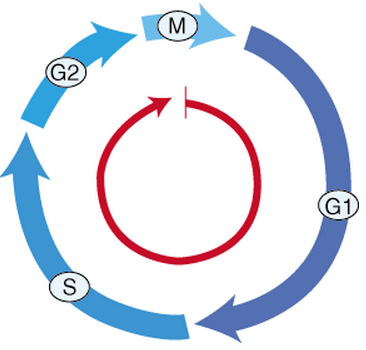
\includegraphics[width=0.3\textwidth]{Images/somaticcellcycle3.png}
\caption{Cell cycle}
\label{cellcycle}
\end{figure}
\end{frame}

\begin{frame}{The raw data}
\begin{columns}[T] % align columns
\begin{column}{.40\textwidth}
\begin{footnotesize}
\begin{figure}[!ht]
\centering
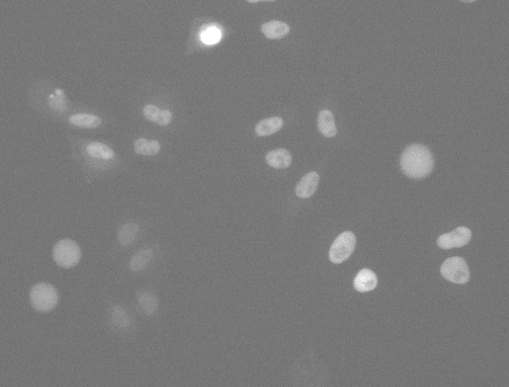
\includegraphics[width=0.50\textwidth]{Images/PCNA.png}
\caption{\textcolor{blue}{Figure :} Data acquired by Michael Olma with the \texttt{PCNA} marker}
\label{PCNA_michael_olma}
\end{figure}
\begin{itemize}
\item Data set that helps us label the data.
\item HeLa cells stably expressing \texttt{PCNA} marker which is informative about the non-mitotic phases.
\end{itemize}
\end{footnotesize}
\end{column}%
\hfill%
\begin{column}{.56\textwidth}
\begin{footnotesize}
\begin{figure}[!ht]
\centering
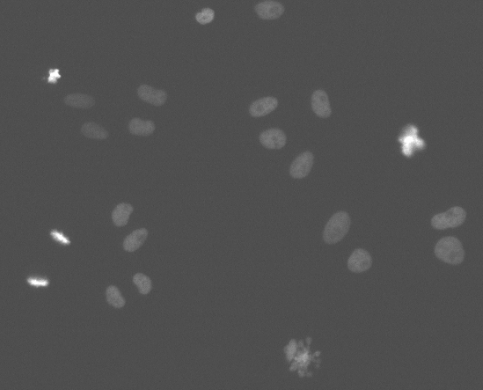
\includegraphics[width=0.38\textwidth]{Images/H2B.png}
\caption{\textcolor{blue}{Figure :} Data acquired by Michael Olma with the \texttt{H2B} marker}
\label{H2B}
\end{figure}
\begin{itemize}
\item Data set from which we extract features for training purposes. 
\item Looking for paterns that help differenciate non-mitotic phases.
\item HeLa cells stably expressing \texttt{H2B} marker, informative about the mitotic phases.
\end{itemize}
\end{footnotesize}
\end{column}%
\end{columns}
\end{frame}

\begin{frame}{Extracting the data}

Using \textit{CellCognition}:
\begin{figure}[!ht]
\centering
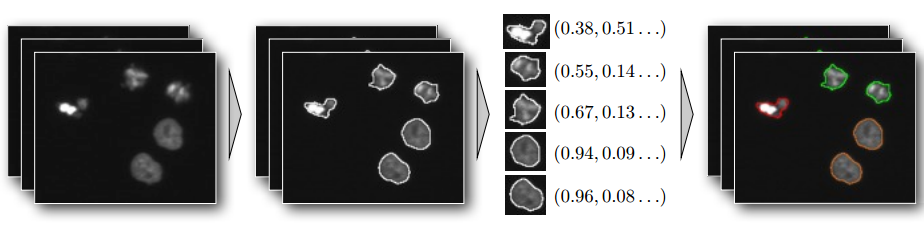
\includegraphics[width=\textwidth]{Images/features_extract.png}
\caption{\textit{CellCognition} steps for feature extraction}
\label{extract}
\end{figure}
\end{frame}

\begin{frame}{Results on the cell cycle phases length}
\begin{footnotesize}
To assess our predicition, we looked at different cell cycle phases length out of 234 trajectories:
\begin{table}[!ht]
\centering
\begin{tabular}{|c|c|c|c|}
  \hline
  Length of:  & Mean & Standard deviation & Number of trajectories \\
  \hline
\text{G1} & 7.13 & 3.8 & 159 \\
  \hline
\text{S}  & 6.28 & 2.9 & 124 \\
  \hline
\text{G2} & 3.17 & 1.4 & 124 \\
  \hline
\text{Cell Cycle} & 16.7 & 4.1 & 124 \\
  \hline 
\end{tabular} 
  \caption{On Michael Olma set with the PCNA channel, our "ground truth"}
\end{table}
\begin{table}[!ht]
\begin{tabular}{|c|c|c|c|}
  \hline
  Length of:  & Mean & Standard deviation & Number of trajectories \\
  \hline
\text{G1} & 6.92 & 3.6 & 164 \\
  \hline
\text{S}  & 8.30 & 3.1 & 102 \\
  \hline
\text{G2} & 1.77 & 2.2 & 102 \\
  \hline
\text{Cell Cycle} & 17.1 & 2.1 & 102 \\
  \hline 
\end{tabular} 
  \caption{On Michael Olma set with the H2B channel}
\end{table}
\end{footnotesize}
\end{frame}

\section{Phd Subject}
%Here I will talk about my phd subject
%%% 3 frames approx

\begin{frame}{Title}
Super text
\end{frame}


\section{Tissue segmentation}
%% I will talk about the challenge, challenging work, novel features, annotated data
%% approx 6 slides
\begin{frame}{Title}
Super text
\end{frame}

\section{Current work}
%% I will talk about my current work + data F.Reyal
%% 6/7 slides approx
\begin{frame}{Title}
Super text
\end{frame}

\section{•}


\begin{frame}{Camelyon16}{ISBI-2016}

\begin{figure}[!ht]
\centering

\includegraphics[width=\textwidth]{Camelyon16.png}
\caption{Official logo}
\label{Ol}
\end{figure}
Challenge apart of ISBI 2016. \\
\textcolor{red}{Important date}:
\begin{itemize}
\item 1st April 2016, submission deadline.
\item 13th to 16th April: ISBI 2016.
\end{itemize}
\end{frame}

\begin{frame}{Camelyon16}

\begin{columns}[T] % align columns
\begin{column}{.50\textwidth}
\begin{small}
\textcolor{red}{Goal:}
\begin{itemize}
\item Detection of micro- and macro-metastases in lymph node digitized images.
\item Automated detection of metatases in hematoxylin and eosin (H\&E) stained whole-slide images of lymph node sections.
\end{itemize}
\textcolor{red}{Motivation:}
\begin{itemize}
\item Lymph node metastases occur in most cancer types.
\item Lymph nodes in the underarm are the first place cancer is likely to spread.
\item The prognosis is poorer when cancer has spread there.
\end{itemize}
\end{small}
\end{column}%
\hfill%
\begin{column}{.50\textwidth}
\begin{figure}[!ht]
\centering
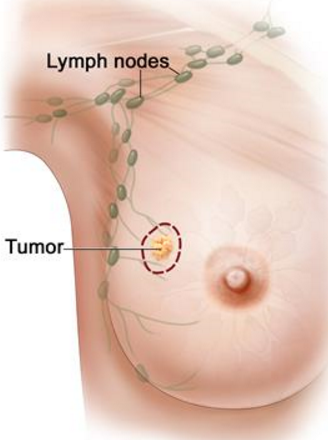
\includegraphics[width=\textwidth]{Booby.png}
\label{booby}
\end{figure}
\end{column}%
\end{columns}

\end{frame}

\begin{frame}{Camelyon16}

\begin{columns}[T] % align columns
\begin{column}{.50\textwidth}
\begin{small}
\textcolor{red}{Goal:}
\begin{itemize}
\item Detection of micro- and macro-metastases in lymph node digitized images.
\item Automated detection of metastases in hematoxylin and eosin (H\&E) stained whole-slide images of lymph node sections.
\end{itemize}
\end{small}
\begin{figure}[!ht]
\centering
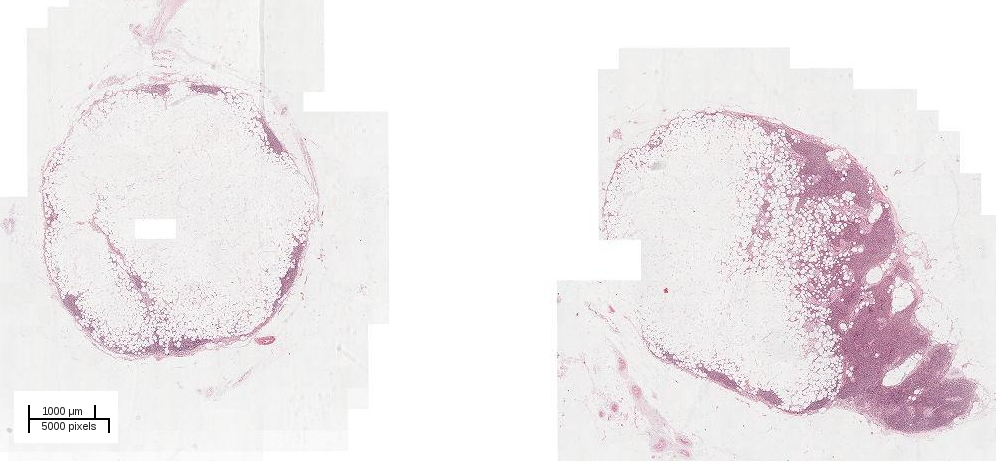
\includegraphics[width=\textwidth]{Normal_38.png}
\caption{Normal 38}
\label{normal_38}
\end{figure}
\end{column}%
\hfill%
\begin{column}{.50\textwidth}
\begin{figure}[!ht]
\centering
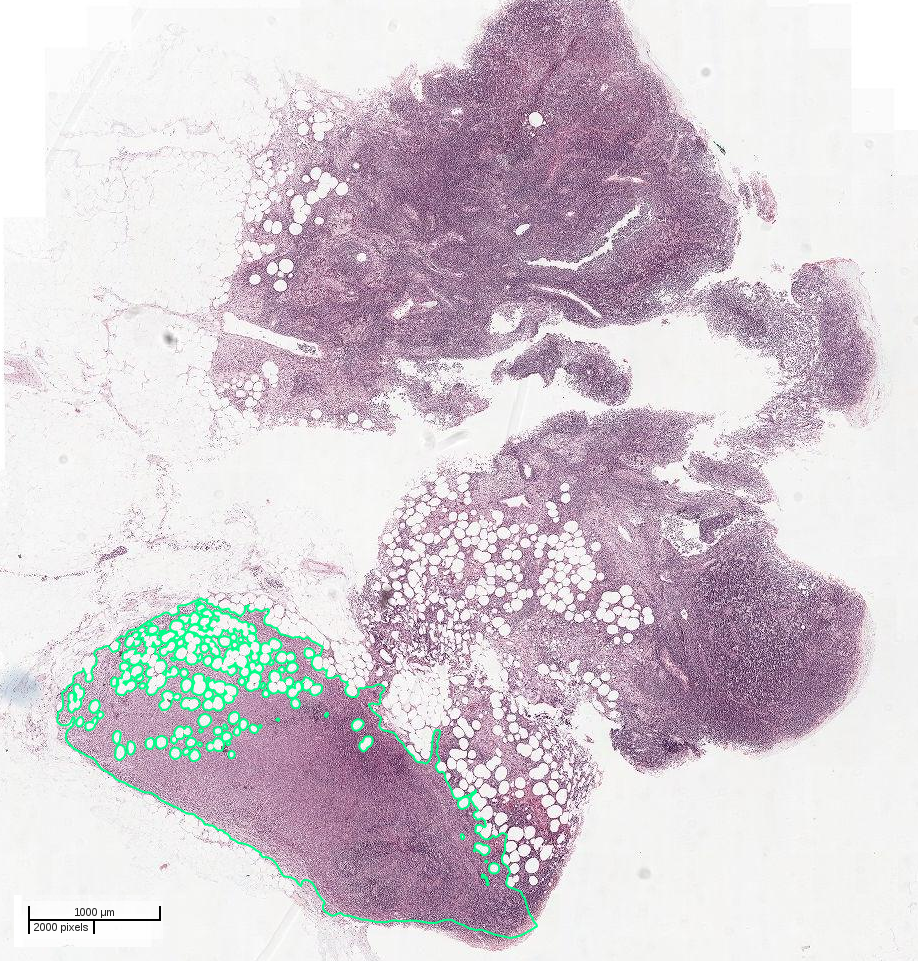
\includegraphics[width=\textwidth]{Tumor_34.png}
\caption{Tumor 34}
{\footnotesize \textit{Metastases detected in green}}
\label{tumor_34}
\end{figure}
\end{column}%
\end{columns}

\end{frame}

% You can reveal the parts of a slide one at a time
% with the \pause command:
\begin{frame}{Evaluation}
Two evaluation metrics and two leader boards. \\
\textcolor{red}{Slides based:}
\begin{itemize}
\item Binary classification of whether or not a slide contains metastases. \item Evaluating with the area under the ROC curve. 
%\item Model:  Multiple Instance Learning models, with a random forest or support vector machine.
\end{itemize}
\textcolor{red}{Region based:}
\begin{itemize}
\item Correctly detecting metastases within slides.
\item Evaluation with the FROC curve (free-response receiver operating characteristic)
%\item Pixel binary classification where a pixel will be labelled "Metastasis" if this pixel belongs to a metastasis.
\end{itemize}
\end{frame}

\section{Technical difficulties}

\subsection{Large Tiff files}

\begin{frame}{The data set}
\begin{columns}[T] % align columns
\begin{column}{.5\textwidth}
Data set provided:
\begin{itemize}
\item 160 Normal slides.
\item 110 Tumor slides.
\end{itemize} 

\begin{small}

\begin{itemize}
\item [--] Huge images with very high precisions, using c++ library openslide. 
\item [--] One image compressed with JPEG2000: $\sim$ 2/3Gb. 
\item [--] Uncompressed at approx. 10Gb. 
\item [--] Highest resolution : $\sim 96 256\times 218624$.
\item [--] Lowest resolution : $\sim 188 \times 427$. 
\end{itemize}
\end{small}

\end{column}%
\hfill%
\begin{column}{.5\textwidth}
\begin{figure}[!ht]
\centering
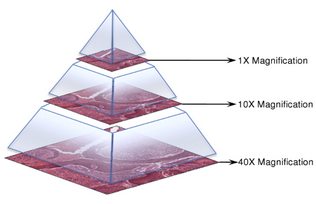
\includegraphics[width=\textwidth]{pyramid.png}
\caption{Pyramid data structure}
\textit{Between 8 and 10 different resolutions}
\label{}
\end{figure}
\end{column}%
\end{columns}

\end{frame}

\begin{frame}{Example}
\begin{columns}[T] % align columns
\begin{column}{.3\textwidth}
\begin{figure}[!ht]
\centering
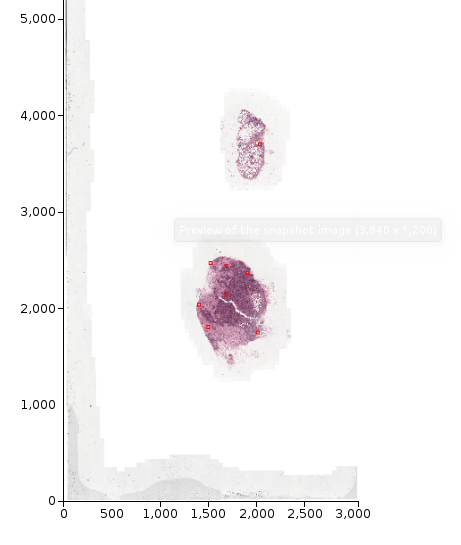
\includegraphics[width=\textwidth]{Tumor_31.png}
\caption{Tumor 31}
\textit{7000 x 3500, resolution 6}
\label{}
\end{figure}
\end{column}%
\hfill%
\begin{column}{.3\textwidth}
\begin{figure}[!ht]
\centering
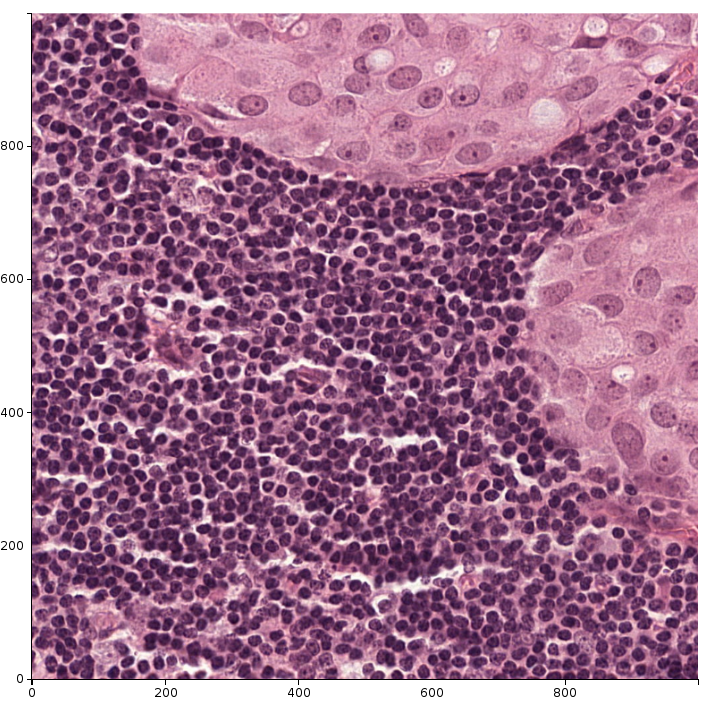
\includegraphics[width=\textwidth]{Tumor_31_res0.png}
\caption{Sub-image of Tumor 31, highest resolution}
\textit{1000 x 1000, resolution 0}
\label{}
\end{figure}
\end{column}%
\hfill%
\begin{column}{.3\textwidth}
\begin{figure}[!ht]
\centering
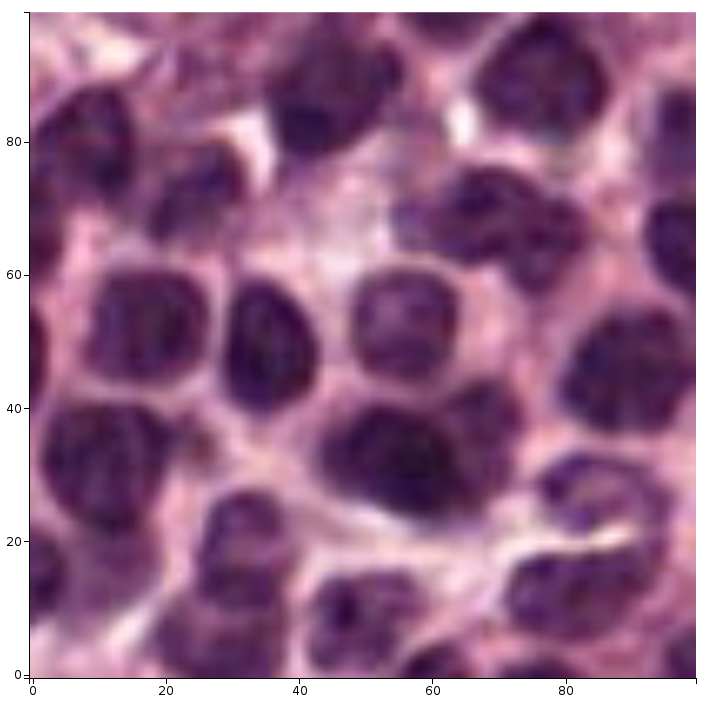
\includegraphics[width=\textwidth]{Tumor_31_res0_zoom.png}
\caption{Sub-image of Tumor 31, highest resolution (zoom)}
\textit{100 x 100, resolution 0}
\label{}
\end{figure}
\end{column}%
\end{columns}
\end{frame}

\subsection{Difficulties linked to imaging}

\begin{frame}{Images}
\textcolor{red}{Very large number of samples:}
\begin{itemize}
\item In pixel classification, each pixel is an instance, n $\gg$ p.
\item Appropriate subsampling methods. In particular here, first subsampling for the "sub-images". Second subsampling given a particular "sub-image".
\end{itemize}
\end{frame}

\section{Workflow}

\subsection{Summary}
\begin{frame}{Summary}
Their was a workflow graph
\end{frame}

\subsection{Subsampling 1}
\begin{frame}{Subsampling}
\textcolor{red}{Subsampling 1} (region of interest detection over slides)
Trying to find interesting part of the image. \\
We can divide sub-images in 4 groups.
\begin{itemize}
\item Only metastasis tissue.
\item Only normal tissue.
\item Centered on the boarder metastasis tissue/normal tissue.
\item Centered on the boarder tissue/background.
\end{itemize}
\end{frame}
\begin{frame}{Subsampling}

\begin{columns}[T] % align columns
\begin{column}{.25\textwidth}
\begin{figure}[!ht]
\centering
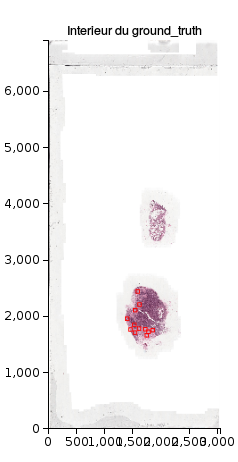
\includegraphics[width=\textwidth]{OnlyPositive.png}
\caption{Only metastasis regions}
\label{}
\end{figure}
\end{column}%
\begin{column}{.25\textwidth}
\begin{figure}[!ht]
\centering
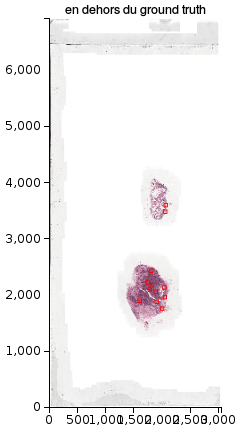
\includegraphics[width=\textwidth]{OnlyNormal.png}
\caption{Only metastasis-free regions}
\label{}
\end{figure}
\end{column}%
\begin{column}{.25\textwidth}
\begin{figure}[!ht]
\centering
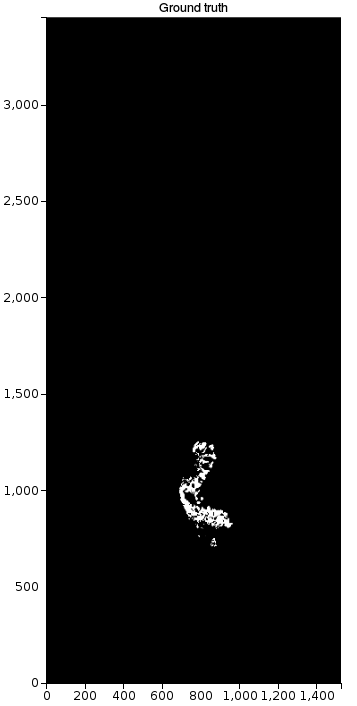
\includegraphics[width=\textwidth]{GT.png}
\caption{Ground truth}
\label{}
\end{figure}
\end{column}%
\begin{column}{.25\textwidth}
\begin{figure}[!ht]
\centering
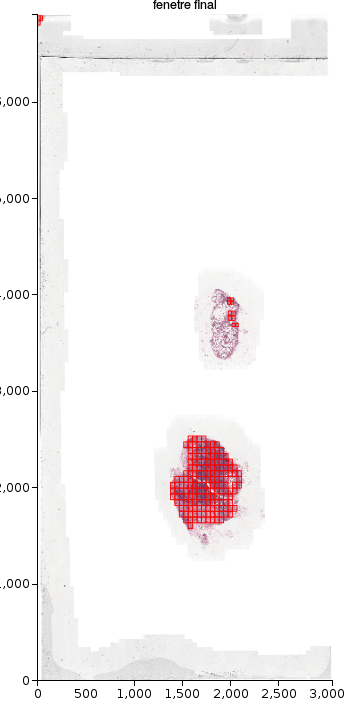
\includegraphics[width=\textwidth]{Grid.png}
\caption{Grid partition}
\label{}
\end{figure}
\end{column}%
\end{columns}
\end{frame}

\subsection{Ilastik features}

\begin{frame}{Ilastik}
\begin{columns}[T] % align columns
\begin{column}{.8\textwidth}

Ilastik : software for interactive image classification, segmentation and analysis. \\
Using features from ilastik (implemented in vigra, c++ library)
\begin{itemize}
\item Color/Intensity:
\begin{itemize}
\item [--] Gaussian Smoothing
\end{itemize}
\item Edge:
\begin{itemize}
\item [--] Laplacian of Gaussian
\item [--] Difference of Gaussians
\item [--] Gaussian Gradiant Magnitude
\end{itemize}
\item Texture:
\begin{itemize}
\item [--] Structure Tensor Eigenvalues
\item [--] Hessian of Gaussian Eigenvalues
\end{itemize}
\end{itemize}
\end{column}%
\begin{column}{.2\textwidth}
\begin{figure}[!ht]
\centering

\includegraphics[width=\textwidth]{Ilastik.png}
\caption{Ilastik}
\label{}
\end{figure}
\end{column}%
\end{columns}
\end{frame}

\begin{frame}{Ilastik - examples}
\begin{columns}[T] % align columns
\begin{column}{.8\textwidth}
\begin{figure}[!ht]
\centering
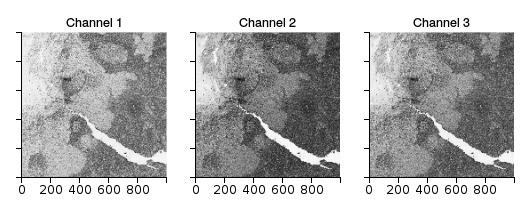
\includegraphics[width=.7\textwidth]{part3_sub1.png}
\caption{Gaussian smoothing, $\sigma=0.7$}
\label{}
\end{figure}
\begin{figure}[!ht]
\centering
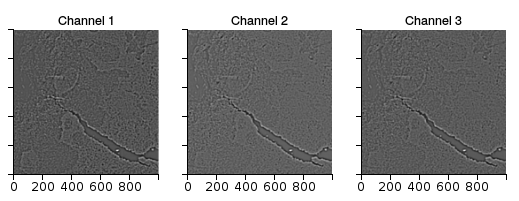
\includegraphics[width=.7\textwidth]{part3_sub2.png}
\caption{Laplacian of Gaussian, $\sigma=5$}
\label{}
\end{figure}
\end{column}%
\begin{column}{.2\textwidth}
\begin{figure}[!ht]
\centering

\includegraphics[width=\textwidth]{Ilastik.png}
\caption{Ilastik}
\label{}
\end{figure}
\end{column}%
\end{columns}
\end{frame}

\subsection{Superpixels/Waterpixels based features}

\begin{frame}{Superpixels/Waterpixels}
Superpixels: Regions resulting from a low-level segmentation. 
They have these proprieties: \textcolor{red}{homogeneity, connected partitions, adherence to object boundaries, regularity}.
\begin{figure}[!ht]
\centering
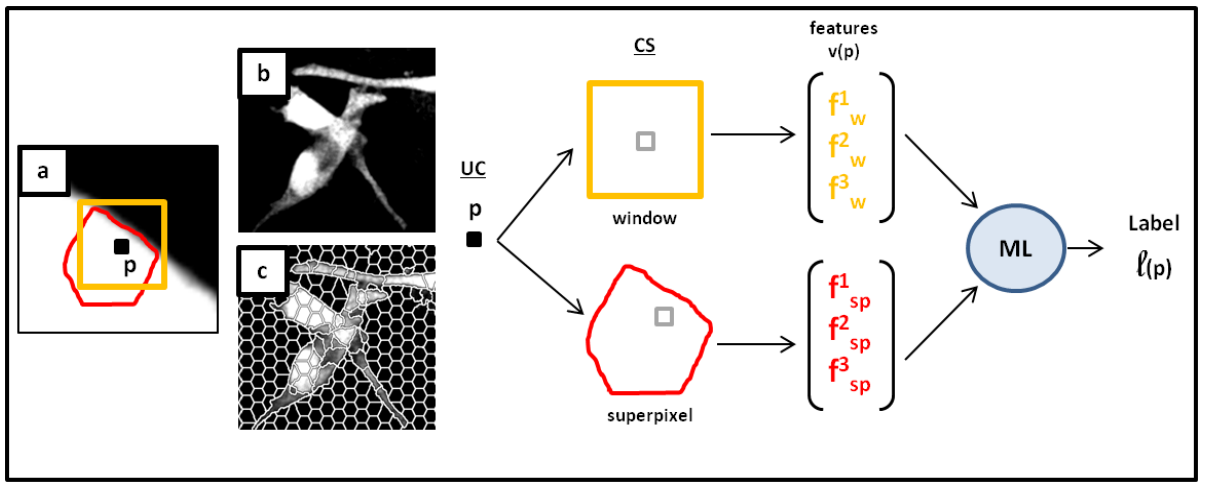
\includegraphics[width=\textwidth]{Waterpixels.png}
\caption{Illustration of how superpixels are used}
\label{}
\end{figure}
\begin{small}
\textcolor{green}{Paper}: \textit{Waterpixels}, V. Machairas, M. Faessel, D. Cardenas-Pena, T. Chabardes, T. Walter and E. Decencière.
\end{small}
\end{frame}

\begin{frame}{Waterpixels - examples}
\begin{columns}[T] % align columns

\begin{column}{.3\textwidth}
\begin{figure}[!ht]
\centering
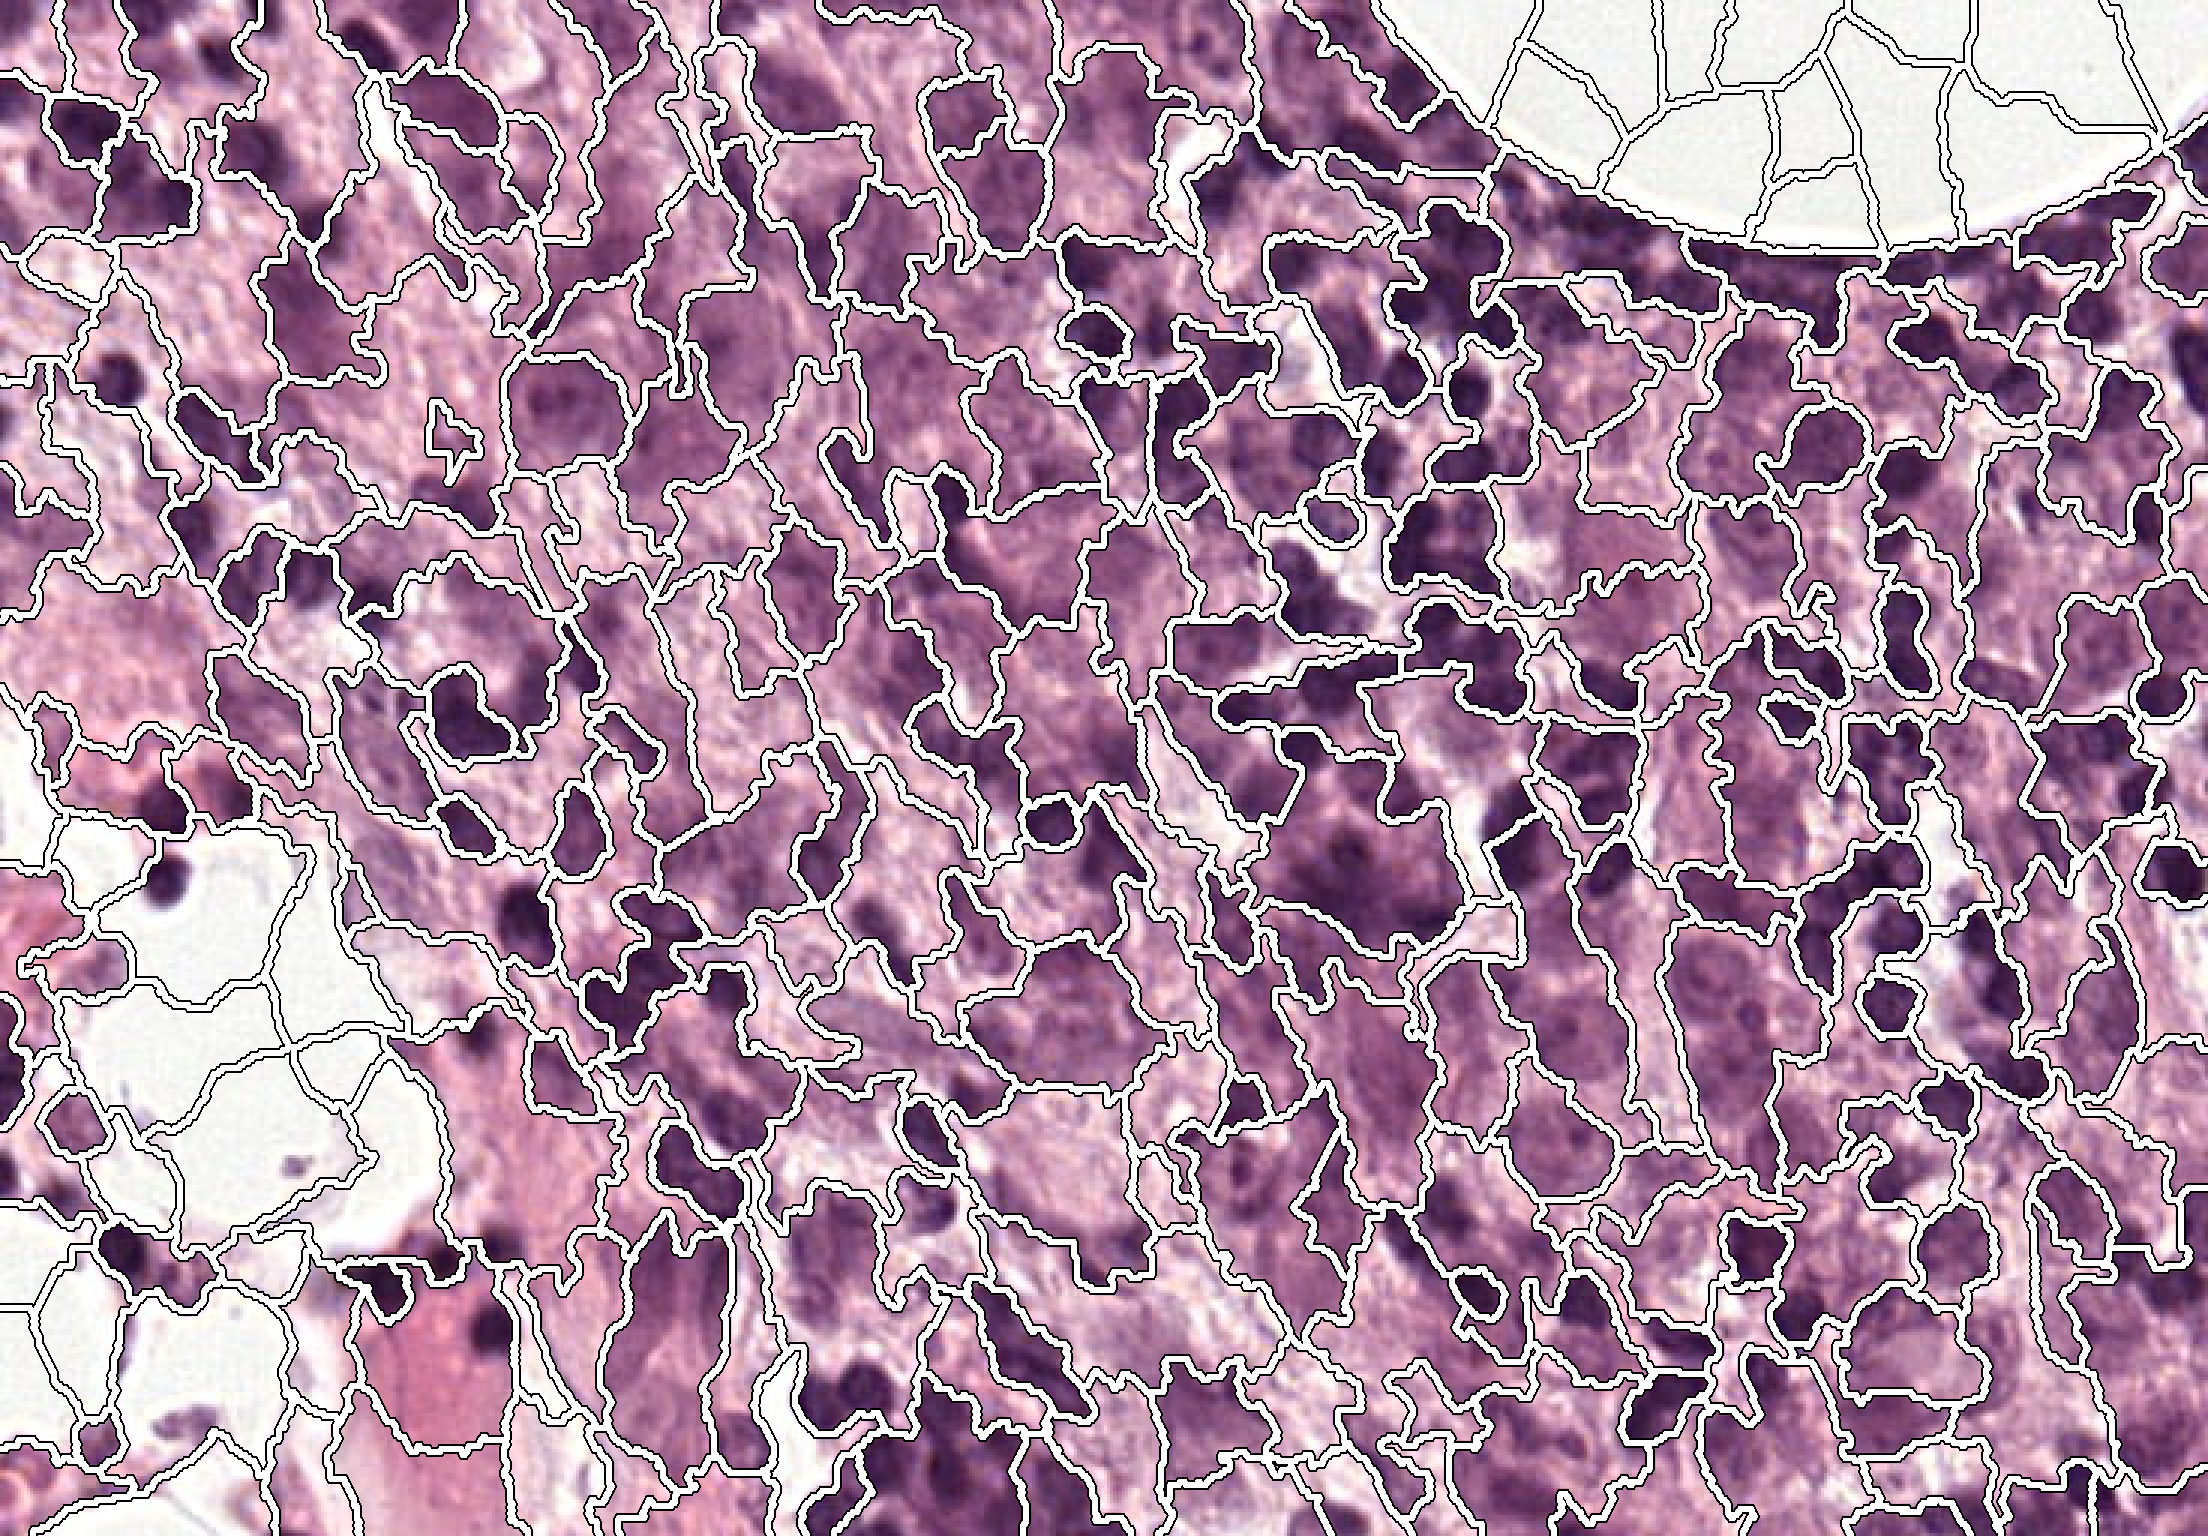
\includegraphics[width=\textwidth]{waterpix_res0.png}
\caption{Waterpixels at resolution 0}
\label{}
\end{figure}
\end{column}%

\begin{column}{.3\textwidth}
\begin{figure}[!ht]
\centering
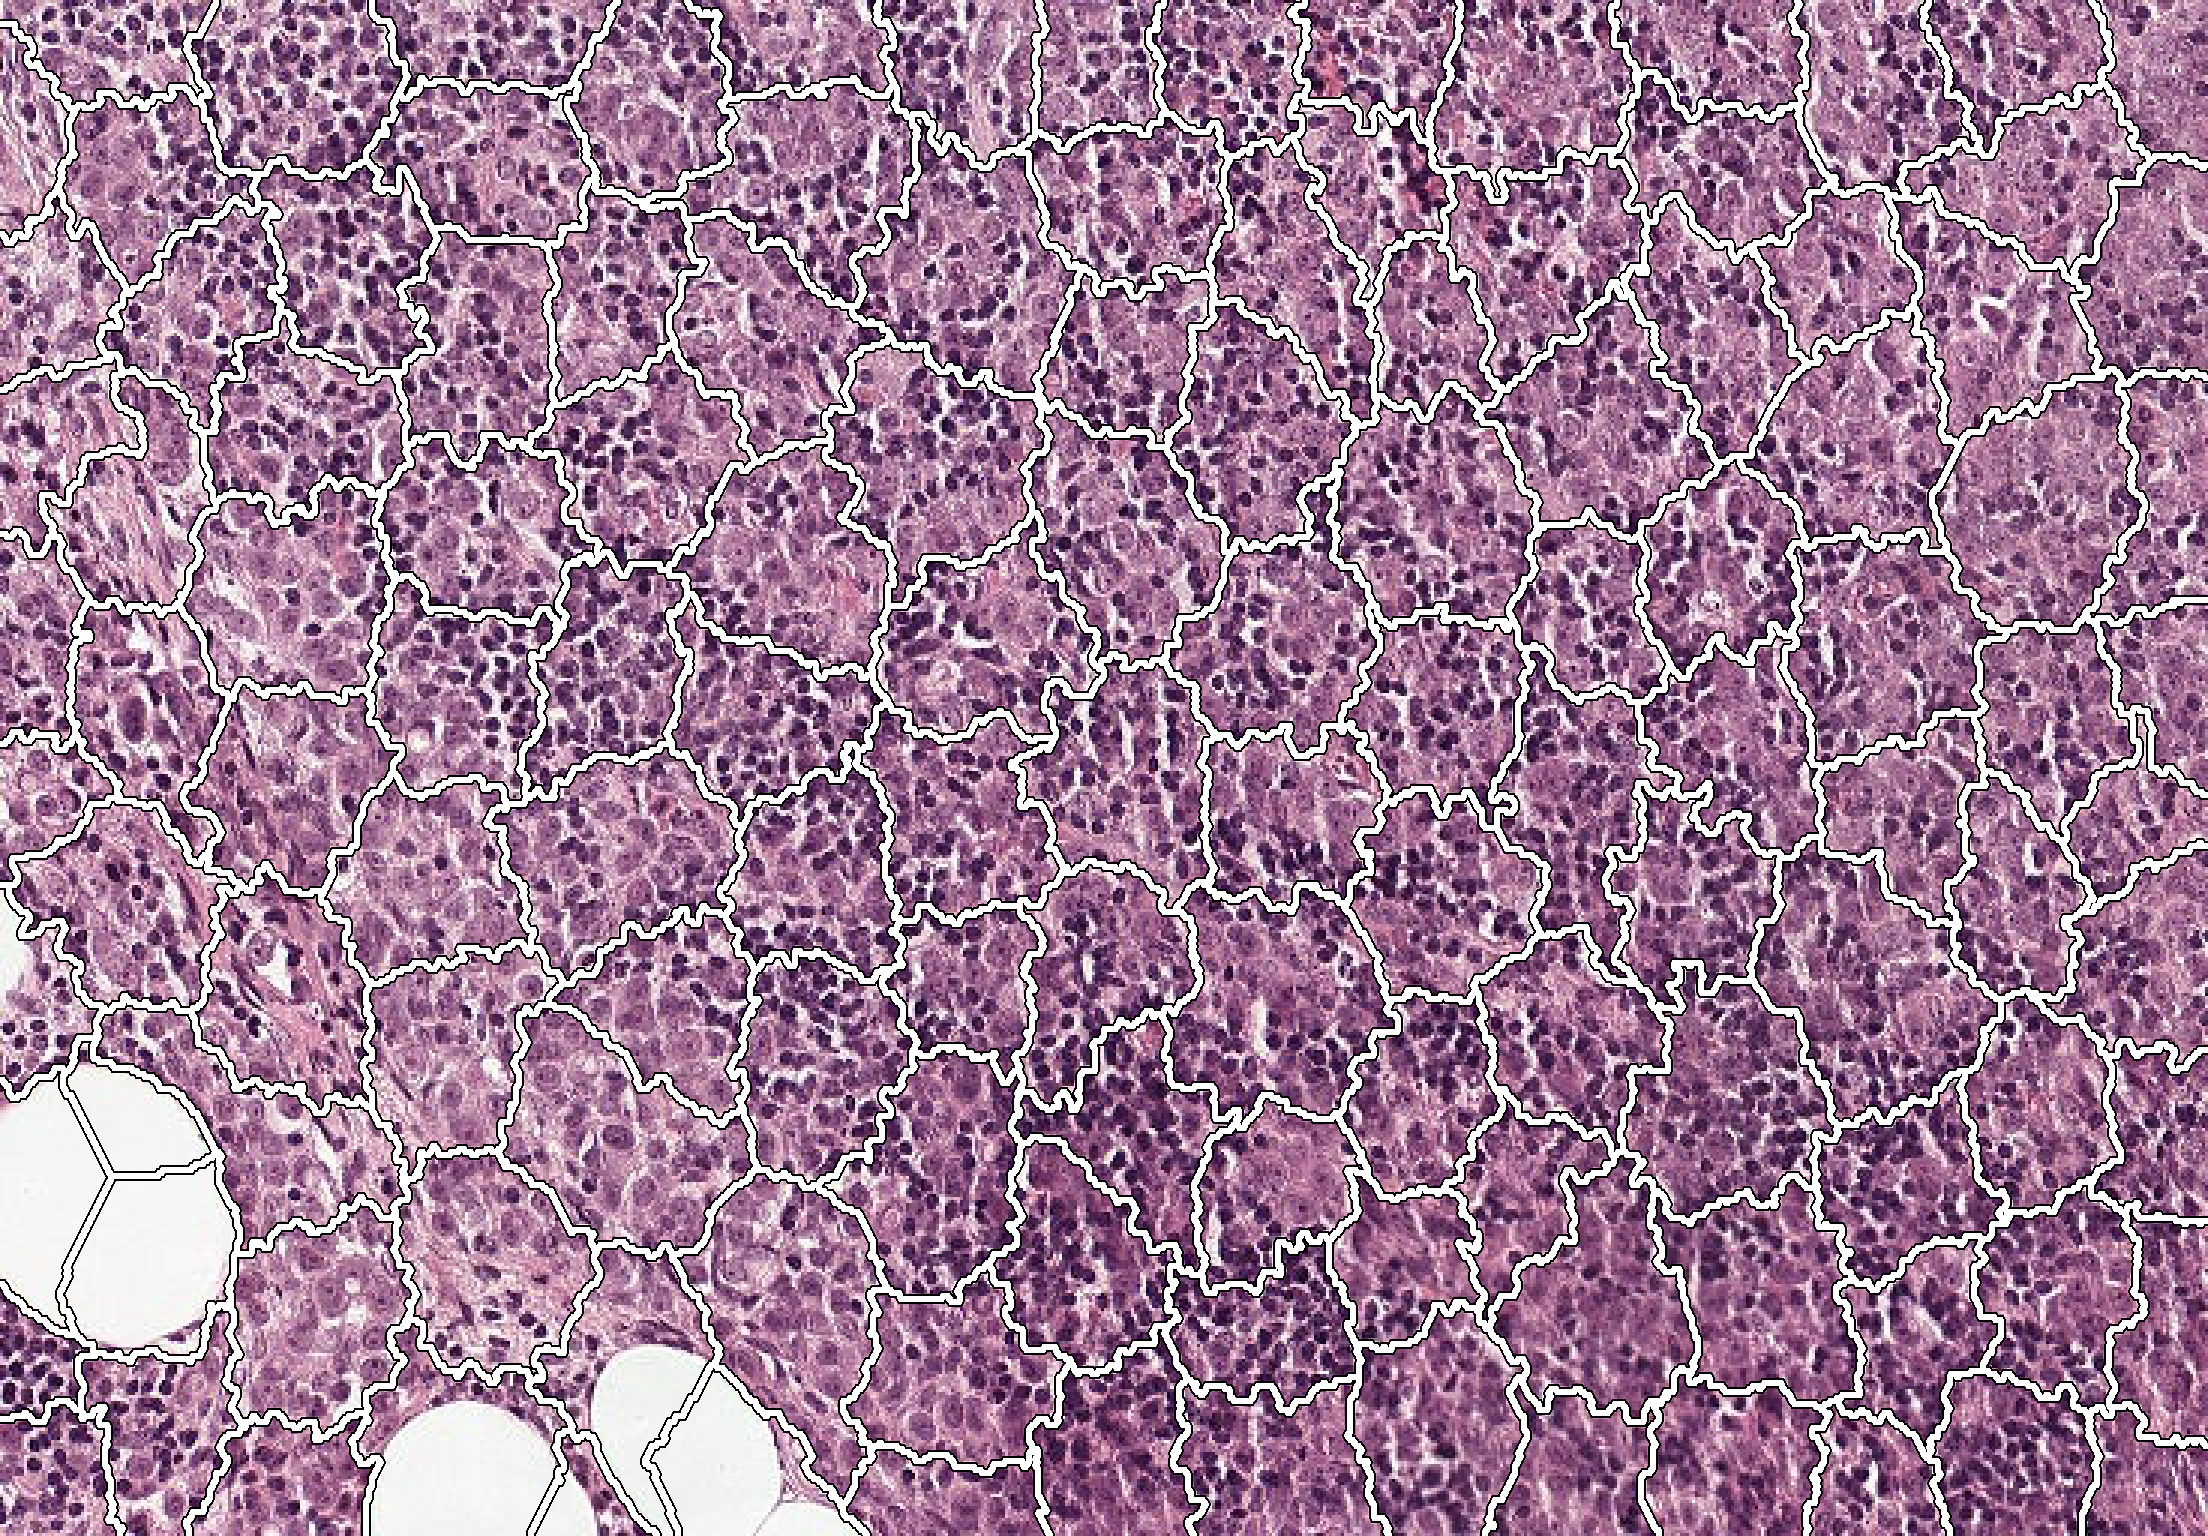
\includegraphics[width=\textwidth]{waterpix_res2.png}
\caption{Waterpixels at resolution 2}
\label{}
\end{figure}
\end{column}%

\begin{column}{.3\textwidth}
\begin{figure}[!ht]
\centering
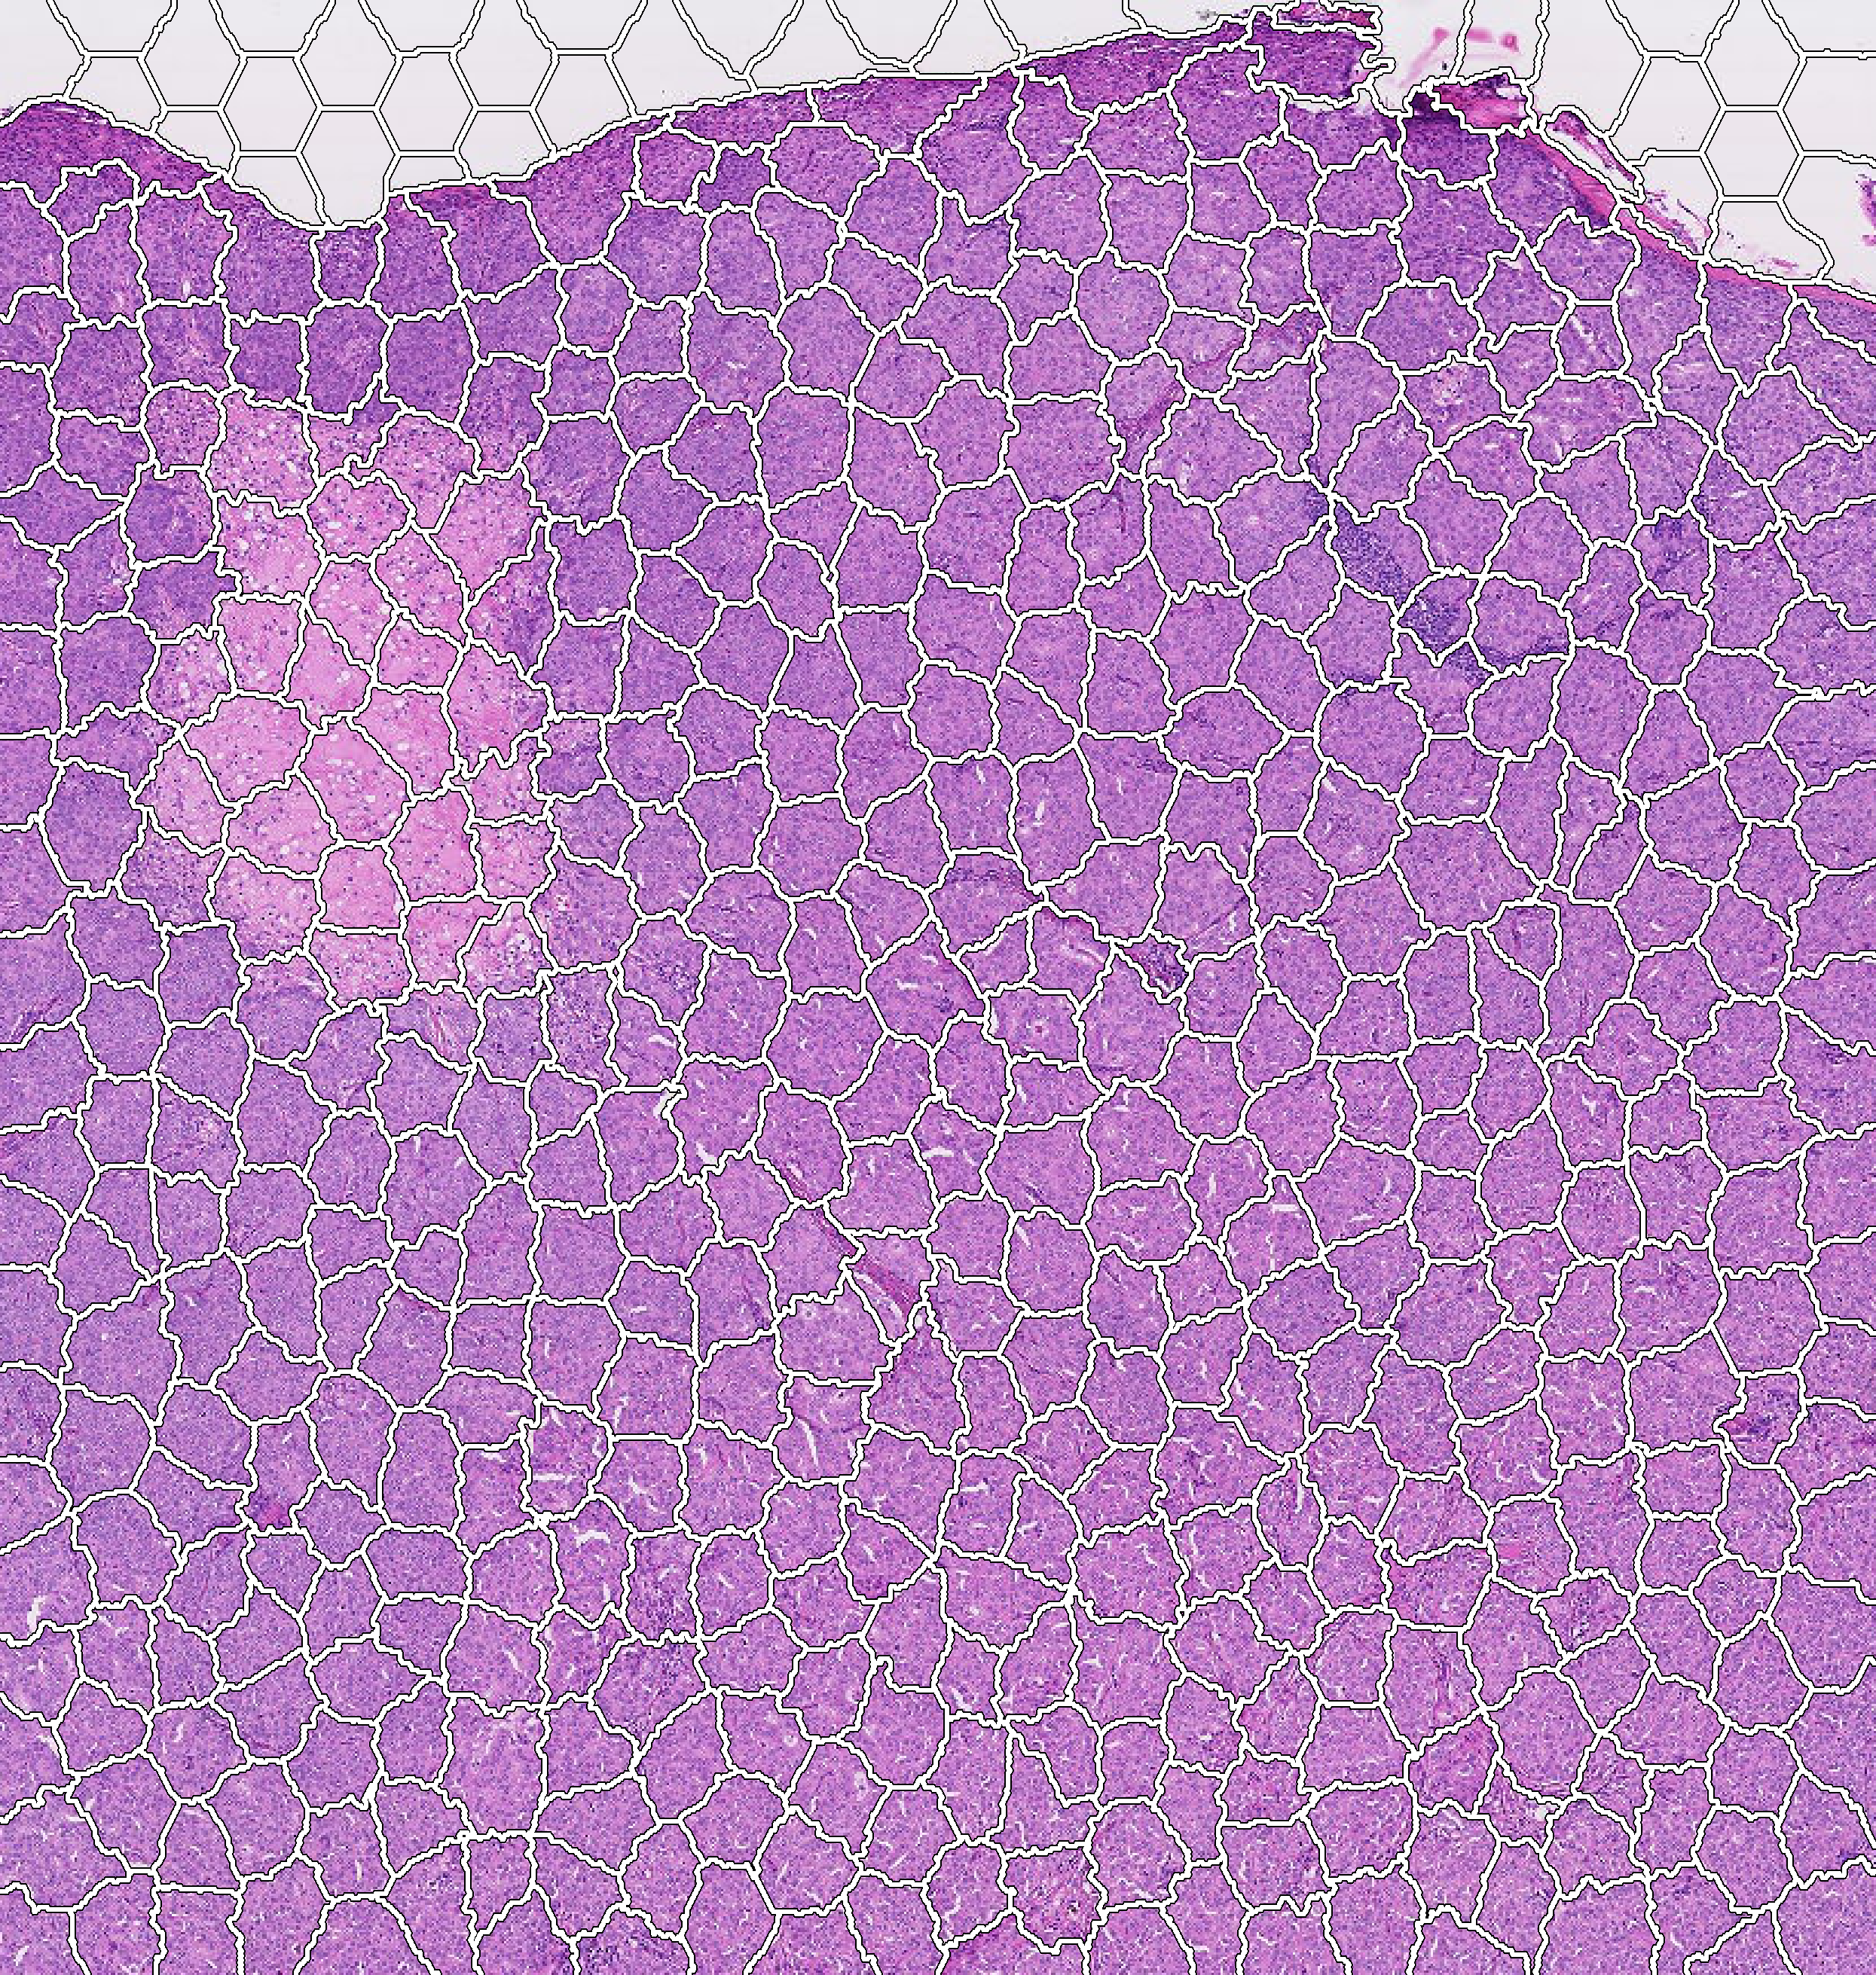
\includegraphics[width=\textwidth]{waterpix_res4.png}
\caption{Waterpixels at resolution 4}
\label{}
\end{figure}
\end{column}%

\end{columns}
\end{frame}

\subsection{Subsampling 2}
\begin{frame}{Subsampling 2}
\textcolor{red}{Pixel classification}. \\
Still very large data-set. \\
260 slides $\rightarrow$ 100 sub-images per slides $\rightarrow$ 1 000 000 pixels per sub-images. \\
Need for a second resampling. \\
Resampling randomly? smartly, via unsupervised methods?
\end{frame}

\subsection{Machine learning}

\begin{frame}{Pixel based classifier}
\textcolor{red}{Finding metastasis regions:}\\
Each pixel, will be considered metastasis if it belongs to a metastasis region. \\
Model: random forest. \\
\textcolor{red}{Detecting metastasis patients:}
Each pixel is or not a metastasis but it also belongs to bigger group. This larger group, the slide, is annotated. \\
Model: Multiple instance learning random forest.
\textcolor{red}{Cross-validation/evaluation:} \\
One slide out scheme.
\end{frame}

\begin{frame}{Multiple instance learning}
\textcolor{red}{Notations}:
\begin{itemize}
\item Pixels are a pair $(x_i,y_i) \in \mathbb{R}^d \times \lbrace -1, +1\rbrace$.
\item Slides are bags of pixels: $B_I=\lbrace x_i, i\in I \rbrace$, and we have $Y_I=1$ if there is at least one $x_i$ in $B_I$ that is positive, otherwise $Y_I=-1$. 
\item \textcolor{red}{Constraint to add} to an optimization problems: \\
$$\sum \frac{y_i+1}{2} \geqslant 1, \forall I \ s.t \ Y_I=1 \ \text{and} \ y_i=-1, \forall I \ s.t \ Y_I=-1$$
\end{itemize}
\textcolor{green}{Implementation} : MISVM, Multiple-Instance Support Vector Machines by Gary Doran. Python package. \\
\textcolor{green}{Paper}: \textit{Support Vector Machines for Multiple Instance learning}, S. Andrews, I. Tsochantaridis and T. Hofmann.
\end{frame}



\end{document}


